\documentclass[11pt,letterpaper]{article}

\usepackage[margin=1in]{geometry}
\usepackage{amsmath,amssymb}
\usepackage{graphicx}
\usepackage{booktabs}
\usepackage{array}
\usepackage{hyperref}
\usepackage{xcolor}
\usepackage{caption}
\usepackage{parskip}

\hypersetup{
  colorlinks=true,
  linkcolor=blue!60!black,
  urlcolor=blue!60!black,
  citecolor=blue!60!black
}

\title{CEC 300 Fixed-Wing Aircraft Pitch Controller Lab Report}
\author{[Gatlin Nelson]}
\date{2026-04-22}

\begin{document}
\maketitle

% =======================================================================
\section{Introduction}

Module 6b introduced classical feedback control as a block diagram: a
reference $r(t)$, a feedback error $e(t)=r(t)-y(t)$ fed into a controller,
and a plant whose output $y(t)$ is compared back against the reference. This
lab applies that structure to a fixed-wing pitch-hold autopilot.

The plant equation derived in Section~2 of the lab guide,
\begin{equation*}
  \frac{d^{2}\theta}{dt^{2}}
  + 0.739\,\frac{d\theta}{dt}
  + 0.921\,\theta(t)
  = 1.15\,\frac{d\delta_{e}}{dt} + 0.17\,\delta_{e}(t),
\end{equation*}
contains two aerodynamic effects on the airplane (left-hand) side:

\begin{itemize}
  \item \textbf{Aerodynamic damping} ($0.739\,d\theta/dt$). The tail acts
  like a shock absorber: as the nose pitches, the tail moves through the
  airstream and the resulting moment opposes the motion, bleeding energy out
  of the rotation.
  \item \textbf{Aerodynamic stiffness / restoring force}
  ($0.921\,\theta$). This is static stability. Any pitch deviation produces
  a moment that pulls the nose back toward the trimmed attitude, which is
  the weathervane analogy used in the lab guide.
\end{itemize}

The right-hand side is the elevator command: a steady elevator deflection
contributes $0.17\,\delta_{e}$, and fast stick motion adds the ``whip'' term
$1.15\,d\delta_{e}/dt$. Taking the Laplace transform gives the plant
transfer function
\begin{equation*}
  G(s) = \frac{1.15\,s + 0.17}{s^{2} + 0.739\,s + 0.921},
\end{equation*}
which the lab guide notes is underdamped ($\zeta \approx 0.37$), so the
aircraft will wobble before settling on a new pitch. The controller $C(s)$
sits in front of $G(s)$ in a unity-feedback loop.

All PID controllers were built with the instructor's corrected coefficient
order \texttt{num = [Kd, Kp, Ki]}, \texttt{den = [1, 0]}, which comes from
writing the controller as a single rational function
\begin{equation*}
  C(s) = K_{p} + \frac{K_{i}}{s} + K_{d}\,s
       = \frac{K_{d}\,s^{2} + K_{p}\,s + K_{i}}{s}.
\end{equation*}

The full simulation is in \texttt{pitch\_control.py}; the metrics table is
cached in \texttt{lab\_data.json}.

% =======================================================================
\section{System Plots}

\begin{figure}[h!]
  \centering
  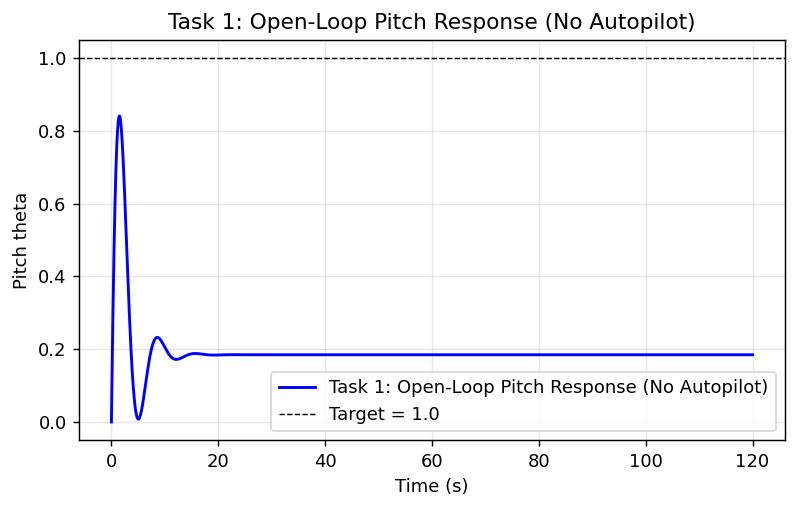
\includegraphics[width=0.78\linewidth]{cec300labimgs/task1_open_loop.png}
  \caption{Task~1: open-loop step response of $G(s)$.}
\end{figure}

\begin{figure}[h!]
  \centering
  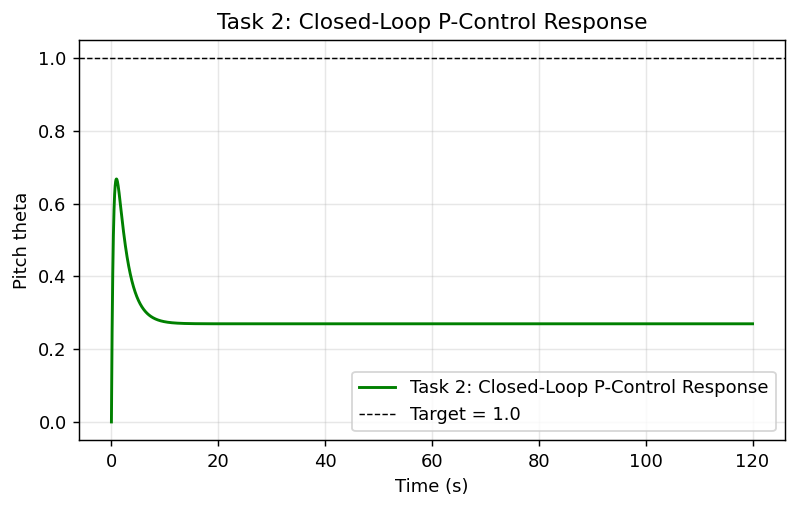
\includegraphics[width=0.78\linewidth]{cec300labimgs/task2_p_control.png}
  \caption{Task~2: closed-loop P-control response, $K_{p}=2$.}
\end{figure}

\begin{figure}[h!]
  \centering
  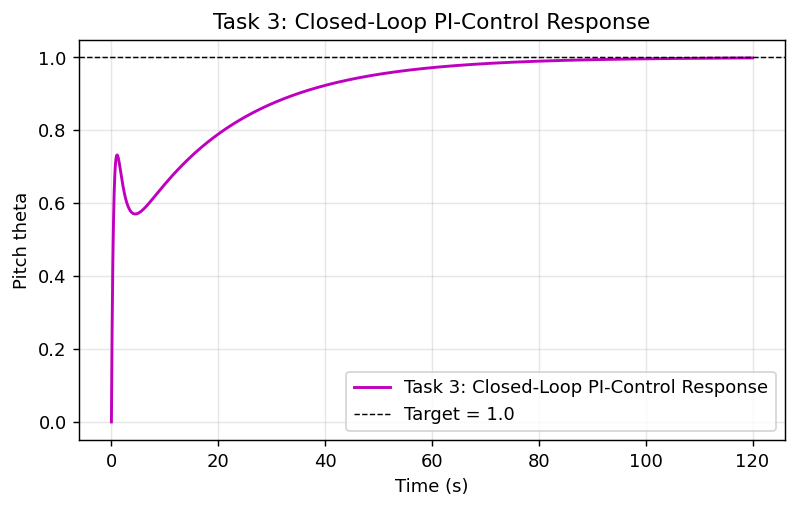
\includegraphics[width=0.78\linewidth]{cec300labimgs/task3_pi_control.png}
  \caption{Task~3: closed-loop PI-control response, $K_{p}=2$, $K_{i}=0.5$.}
\end{figure}

\begin{figure}[h!]
  \centering
  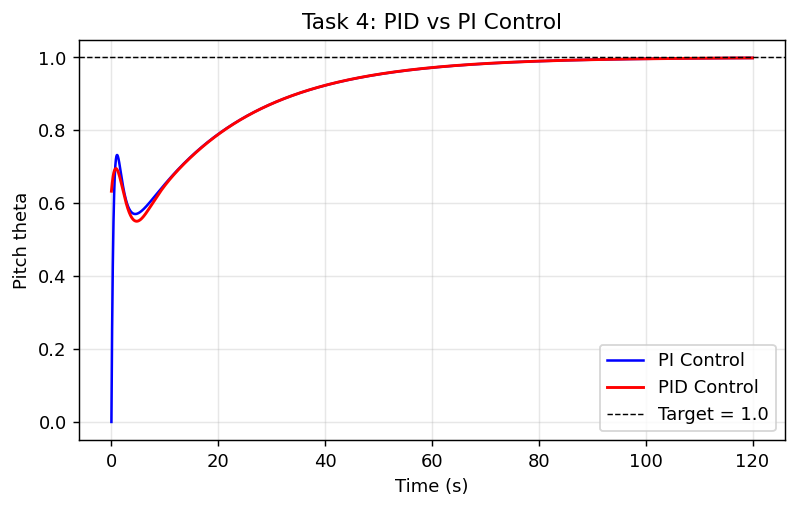
\includegraphics[width=0.78\linewidth]{cec300labimgs/task4_pid_vs_pi.png}
  \caption{Task~4: PID vs PI comparison, $K_{p}=2$, $K_{i}=0.5$, $K_{d}=1.5$.}
\end{figure}

\begin{figure}[h!]
  \centering
  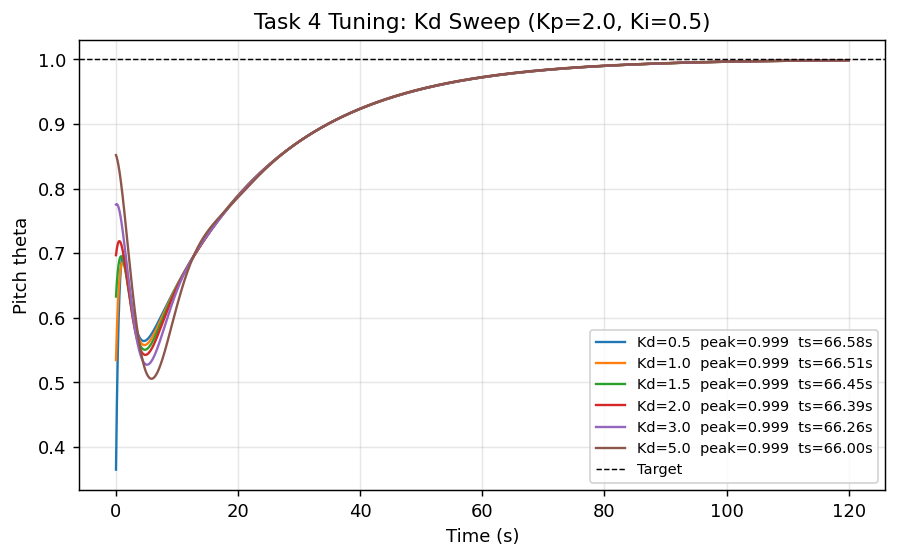
\includegraphics[width=0.85\linewidth]{cec300labimgs/task4_kd_sweep.png}
  \caption{Task~4 tuning: $K_{d}$ sweep at fixed $K_{p}=2$, $K_{i}=0.5$.}
\end{figure}

\clearpage

% =======================================================================
\section{Data Table}

The four columns below correspond to the four tasks: \textbf{Open-Loop} is
the raw plant response with no autopilot; \textbf{P} is the Task~2
proportional controller with $K_{p}=2$; \textbf{PI} is the Task~3
proportional-integral controller with $K_{p}=2$ and $K_{i}=0.5$; and
\textbf{PID} is the Task~4 full controller with $K_{p}=2$, $K_{i}=0.5$, and
$K_{d}=1.5$. Simulation horizon was 120\,s so the integral-dominated
closed-loop responses had time to reach steady state; ``Settle Time'' uses
the 2\,\% criterion.

\begin{table}[h!]
\centering
\small
\begin{tabular}{@{}lcccc@{}}
\toprule
\textbf{Metric} & \textbf{Open-Loop} & \textbf{P} & \textbf{PI} & \textbf{PID} \\
\midrule
Final Value (Steady State) & 0.1846 & 0.2696 & 0.9986 & 0.9987 \\
Steady-State Error         & 0.8154 & 0.7304 & 0.0014 & 0.0013 \\
Peak Value                 & 0.8404 & 0.6675 & 0.9986 & 0.9987 \\
Settle Time (2\,\%)        & n/a    & n/a    & 66.64\,s & 66.45\,s \\
\bottomrule
\end{tabular}
\end{table}

The open-loop and P-control responses never fall within 2\,\% of the
target. The open-loop response levels off at roughly 0.185, because the
plant's DC gain is less than one. P-control does slightly better (0.27)
but still leaves a large steady-state error that pure proportional action
cannot remove. Section~4 explains why.

% =======================================================================
\section{Why $K_{p}$ alone wasn't enough, and how $K_{i}$ fixed it}

With only proportional control, the elevator deflection is proportional to
the feedback error: $\delta_{e} = K_{p}\,e$. A non-zero deflection is needed
to hold the aircraft at a new pitch against the aerodynamic restoring force,
so some error has to remain. Module 6b describes this directly: as the
error shrinks, the proportional push shrinks with it, so the response lands
``near, but not quite at the commanded state.'' With $K_{p}=2$ the response
settled at 0.27, leaving an error of 0.73.

Adding the integral term $K_{i}/s$ accumulates past error over time. Even
when the remaining error is tiny, the integrator keeps driving the elevator
command upward until the error is zero. In the simulation, this dropped the
steady-state error from 0.7304 down to 0.0014, essentially eliminating it.

% =======================================================================
\section{How $K_{i}$ impacted the controller response}

\begin{itemize}
  \item \textbf{Steady-state error:} dropped by roughly 99.8\,\%, going
  from 0.7304 under P-control down to 0.0014 under PI. This was the
  dominant effect, because the integrator accumulates the residual error
  and continues pushing the elevator until the error is gone.
  \item \textbf{Settle time:} under P-control, no meaningful settle time
  existed because the response never came close to the target. Under PI,
  the response finally reaches the 2\,\% band, although it takes 66.64\,s
  to do so.
  \item \textbf{Plot shape:} the initial whip spike (roughly 0.73) is
  similar to the open-loop and P-control transients, but after the natural
  wobble dips back to around 0.58, the integrator slowly winds up and
  carries the response smoothly to 1.0.
\end{itemize}

$K_{i}$ does not itself change the damping of the airframe, because the
aerodynamic damping term (0.739) comes from the plant rather than from the
controller. What $K_{i}$ changes is whether the loop is willing to keep
pushing when the error is small. The cost is a slow approach, since the
integrator at $K_{i}=0.5$ takes time to wind up to the deflection needed to
hold the pitch. Module 6b notes this tradeoff directly: too small a
$K_{i}$ is sluggish, while too large a $K_{i}$ risks overshoot or
oscillation as the integral term outruns the system.

% =======================================================================
\section{How $K_{d}$ impacted the controller response}

The derivative term acts as a dampener, reacting to how fast the error is
changing rather than to the error itself. Module 6b describes its purpose
as limiting the rate of change more as the output reaches the set point,
which mitigates overshoot.

I swept $K_{d}$ across $\{0.5, 1.0, 1.5, 2.0, 3.0, 5.0\}$ with $K_{p}$ and
$K_{i}$ fixed:

\begin{table}[h!]
\centering
\small
\begin{tabular}{@{}ccccc@{}}
\toprule
$K_{d}$ & Final & SS Error & Peak & Settle (2\,\%) \\
\midrule
0.50 & 0.9987 & 0.0013 & 0.9987 & 66.58\,s \\
1.00 & 0.9987 & 0.0013 & 0.9987 & 66.51\,s \\
1.50 & 0.9987 & 0.0013 & 0.9987 & 66.45\,s \\
2.00 & 0.9987 & 0.0013 & 0.9987 & 66.39\,s \\
3.00 & 0.9987 & 0.0013 & 0.9987 & 66.26\,s \\
5.00 & 0.9988 & 0.0012 & 0.9988 & 66.00\,s \\
\bottomrule
\end{tabular}
\end{table}

Observations from the sweep plot:

\begin{itemize}
  \item The \textbf{initial transient spike} at $t\approx0.1$\,s grows with
  $K_{d}$, from roughly 0.37 at $K_{d}=0.5$ up to roughly 0.85 at
  $K_{d}=5.0$. This is because a step input passed through a $K_{d}\,s$
  term produces a large derivative kick, effectively a sudden elevator
  punch.
  \item \textbf{Settle time and final value} barely move across a
  10$\times$ sweep: settle time shortens from 66.58\,s to 66.00\,s, and
  steady-state error improves from 0.0013 to 0.0012.
  \item \textbf{Dampening / overshoot:} there is no overshoot above 1.0 in
  this configuration for any $K_{d}$, so there is nothing for the
  derivative term to damp. The response is integrator-limited rather than
  damping-limited.
\end{itemize}

$K_{d}$ has little to do in this tuning because the base PI loop is
already non-oscillatory. Its role would become meaningful if $K_{p}$ were
raised to tighten the loop, because overshoot would then appear and
$K_{d}$ would suppress it. At the gains specified by the lab, $K_{d}$
mostly just adds an initial control kick without changing the long-term
response.

% =======================================================================
\section{Tuning results}

The assigned gains ($K_{p}=2$, $K_{i}=0.5$, $K_{d}=1.5$) produce an accurate
response ($\mathrm{SSE}\approx 0.001$) but a slow one
($t_{s}\approx 66.5$\,s). Within the specified $K_{d}$ range, the best
settle time I reached was 66.00\,s at $K_{d}=5.0$. The improvement over
$K_{d}=1.5$ is less than 1\,\% (0.45\,s out of 66\,s), and it comes at the
cost of a more aggressive initial control input. The assigned $K_{d}=1.5$
is a reasonable compromise:

\begin{itemize}
  \item Accuracy: $\mathrm{SSE}\approx 0.13\,\%$.
  \item No overshoot above the commanded pitch.
  \item Moderate initial elevator deflection (no sharp kick that would feel
  jerky to passengers).
  \item Settle time $\approx 66.5$\,s (slow, but acceptable for a pitch-hold
  autopilot on a light aircraft where the restoring force is modest).
\end{itemize}

Raising $K_{p}$ (and, proportionally, $K_{i}$) would be the more productive
direction if faster response were needed; $K_{d}$ would then earn its keep
by keeping the tighter loop from ringing.

\medskip
\noindent\textbf{Coefficient values used:} $K_{p}=2$, $K_{i}=0.5$, $K_{d}=1.5$.\\
\textbf{Best observed settle time (assigned gains):} 66.45\,s.

% =======================================================================
\section{Lessons learned}

\begin{enumerate}
  \item \textbf{Proportional control alone cannot reach the target.}
  Module 6b describes the response as landing ``near, but not quite at the
  commanded state,'' and Task~2's final value of 0.27 against a commanded
  pitch of 1.0 made that concrete.
  \item \textbf{Integral action is what eliminates residual error}, and it
  does so by accumulating past error. That is also what makes it slow,
  because the integrator at $K_{i}=0.5$ needed roughly 60\,s to wind up to
  the deflection required to hold pitch.
  \item \textbf{Derivative action only helps when there is something to
  damp.} My $K_{d}$ sweep showed almost no change across a 10$\times$
  range, because the base PI loop already rose monotonically toward 1.0
  without ringing. $K_{d}$'s role is to enable faster tuning, not to be
  useful on its own.
  \item \textbf{Simulation horizon matters.} My first run used a 30\,s
  window and the PI response looked stuck at 0.87, but it was actually
  still climbing. Extending the window to 120\,s showed the integrator
  completing its wind-up and landing on 1.0. This was a good reminder to
  check whether a simulation has actually reached steady state before
  trusting its ``final'' value.
\end{enumerate}

\end{document}
